\documentclass{standalone}
\usepackage{tikz}
\usetikzlibrary{patterns, positioning}

\begin{document}
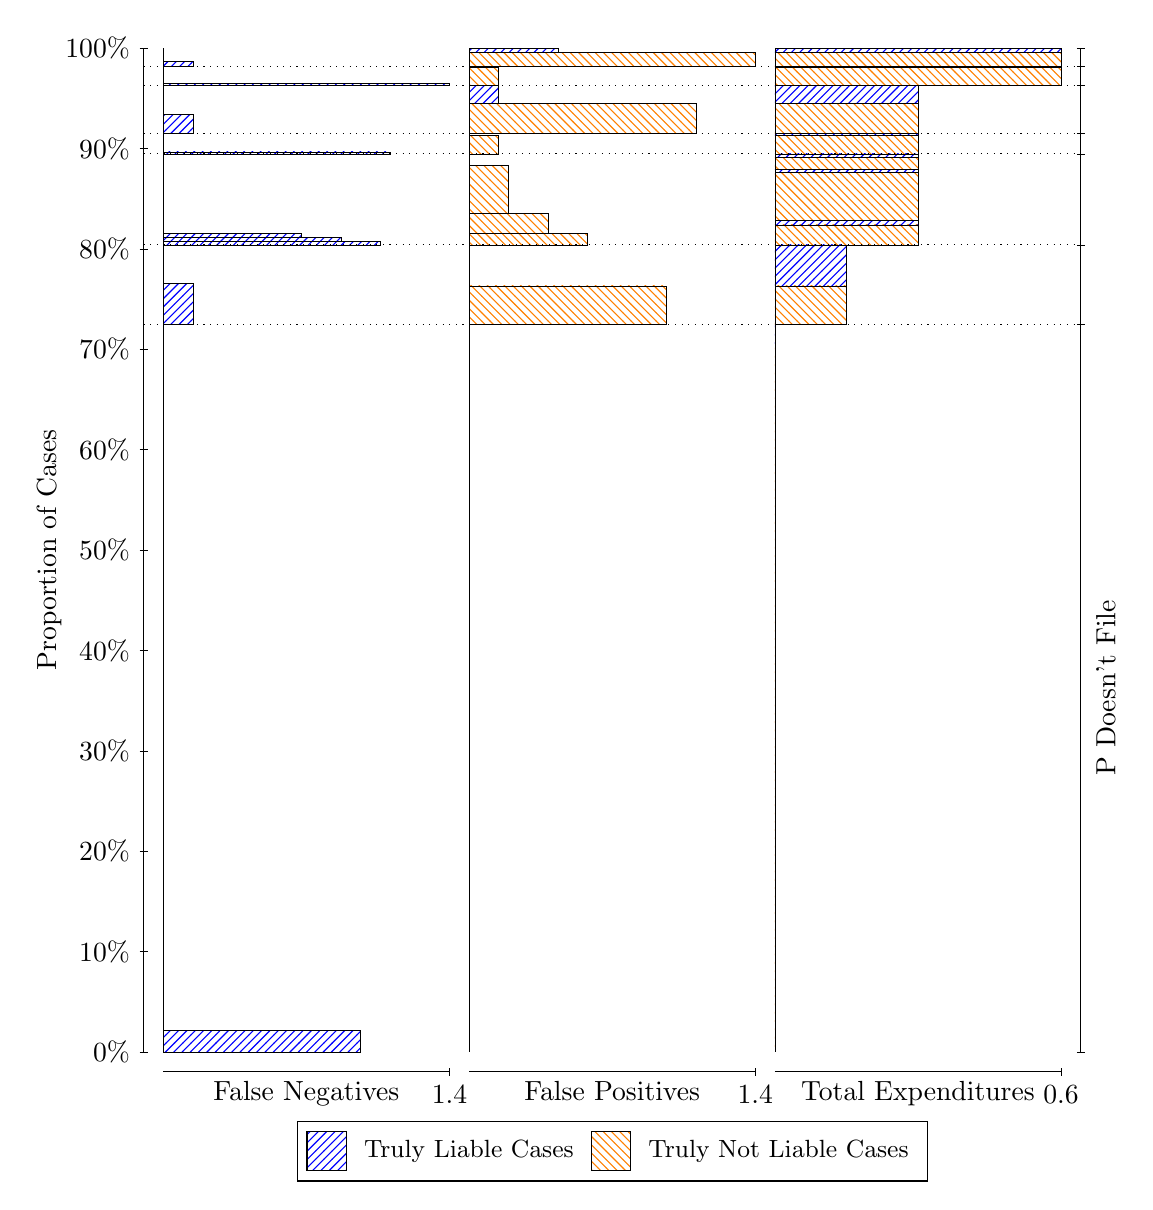
\begin{tikzpicture}
\draw[black, very thin] (1.5,1.75) -- (1.5,14.5);
\node[rotate=90, anchor=center] at (0.3, 8.125) {Proportion of Cases};
\draw[black, very thin] (1.45,1.75) -- (1.55,1.75);
\node[anchor=east] at (1.45, 1.75) {0\%};
\draw[black, very thin] (1.45,3.025) -- (1.55,3.025);
\node[anchor=east] at (1.45, 3.025) {10\%};
\draw[black, very thin] (1.45,4.3) -- (1.55,4.3);
\node[anchor=east] at (1.45, 4.3) {20\%};
\draw[black, very thin] (1.45,5.575) -- (1.55,5.575);
\node[anchor=east] at (1.45, 5.575) {30\%};
\draw[black, very thin] (1.45,6.85) -- (1.55,6.85);
\node[anchor=east] at (1.45, 6.85) {40\%};
\draw[black, very thin] (1.45,8.125) -- (1.55,8.125);
\node[anchor=east] at (1.45, 8.125) {50\%};
\draw[black, very thin] (1.45,9.4) -- (1.55,9.4);
\node[anchor=east] at (1.45, 9.4) {60\%};
\draw[black, very thin] (1.45,10.675) -- (1.55,10.675);
\node[anchor=east] at (1.45, 10.675) {70\%};
\draw[black, very thin] (1.45,11.95) -- (1.55,11.95);
\node[anchor=east] at (1.45, 11.95) {80\%};
\draw[black, very thin] (1.45,13.225) -- (1.55,13.225);
\node[anchor=east] at (1.45, 13.225) {90\%};
\draw[black, very thin] (1.45,14.5) -- (1.55,14.5);
\node[anchor=east] at (1.45, 14.5) {100\%};

\draw[black, very thin] (13.4,1.75) -- (13.4,14.5);
\draw[black, very thin] (13.35,1.75) -- (13.45,1.75);
\node[anchor=west] at (13.35, 1.75) {};
\draw[black, very thin] (13.35,10.993) -- (13.45,10.993);
\node[anchor=west] at (13.35, 10.993) {};
\draw[black, very thin] (13.35,12.001) -- (13.45,12.001);
\node[anchor=west] at (13.35, 12.001) {};
\draw[black, very thin] (13.35,13.155) -- (13.45,13.155);
\node[anchor=west] at (13.35, 13.155) {};
\draw[black, very thin] (13.35,13.42) -- (13.45,13.42);
\node[anchor=west] at (13.35, 13.42) {};
\draw[black, very thin] (13.35,14.029) -- (13.45,14.029);
\node[anchor=west] at (13.35, 14.029) {};
\draw[black, very thin] (13.35,14.271) -- (13.45,14.271);
\node[anchor=west] at (13.35, 14.271) {};
\draw[black, very thin] (13.35,14.5) -- (13.45,14.5);
\node[anchor=west] at (13.35, 14.5) {};

\draw[black, very thin, pattern color=blue, pattern=north east lines] (1.75,1.75) rectangle (4.2557,2.029);
\draw[black, very thin, pattern color=orange, pattern=north west lines] (1.75,2.029) rectangle (1.75,10.993);
\draw[black, very thin, pattern color=blue, pattern=north east lines] (1.75,10.993) rectangle (2.1259,11.514);
\draw[black, very thin, pattern color=orange, pattern=north west lines] (1.75,11.514) rectangle (1.75,12.001);
\draw[black, very thin, pattern color=blue, pattern=north east lines] (1.75,12.001) rectangle (4.5063,12.041);
\draw[black, very thin, pattern color=blue, pattern=north east lines] (1.75,12.041) rectangle (4.0052,12.095);
\draw[black, very thin, pattern color=blue, pattern=north east lines] (1.75,12.095) rectangle (3.504,12.143);
\draw[black, very thin, pattern color=orange, pattern=north west lines] (1.75,12.143) rectangle (1.75,13.155);
\draw[black, very thin, pattern color=blue, pattern=north east lines] (1.75,13.155) rectangle (4.6316,13.18);
\draw[black, very thin, pattern color=orange, pattern=north west lines] (1.75,13.18) rectangle (1.75,13.42);
\draw[black, very thin, pattern color=blue, pattern=north east lines] (1.75,13.42) rectangle (2.1259,13.653);
\draw[black, very thin, pattern color=orange, pattern=north west lines] (1.75,13.653) rectangle (1.75,14.029);
\draw[black, very thin, pattern color=blue, pattern=north east lines] (1.75,14.029) rectangle (5.3833,14.048);
\draw[black, very thin, pattern color=orange, pattern=north west lines] (1.75,14.048) rectangle (1.75,14.271);
\draw[black, very thin, pattern color=blue, pattern=north east lines] (1.75,14.271) rectangle (2.1259,14.326);
\draw[black, very thin, pattern color=orange, pattern=north west lines] (1.75,14.326) rectangle (1.75,14.5);
\draw[black, very thin, pattern color=orange, pattern=north west lines] (5.6333,1.75) rectangle (5.6333,10.714);
\draw[black, very thin, pattern color=blue, pattern=north east lines] (5.6333,10.714) rectangle (5.6333,10.993);
\draw[black, very thin, pattern color=orange, pattern=north west lines] (5.6333,10.993) rectangle (8.1391,11.479);
\draw[black, very thin, pattern color=blue, pattern=north east lines] (5.6333,11.479) rectangle (5.6333,12.001);
\draw[black, very thin, pattern color=orange, pattern=north west lines] (5.6333,12.001) rectangle (7.1368,12.146);
\draw[black, very thin, pattern color=orange, pattern=north west lines] (5.6333,12.146) rectangle (6.6356,12.398);
\draw[black, very thin, pattern color=orange, pattern=north west lines] (5.6333,12.398) rectangle (6.1345,13.013);
\draw[black, very thin, pattern color=blue, pattern=north east lines] (5.6333,13.013) rectangle (5.6333,13.155);
\draw[black, very thin, pattern color=orange, pattern=north west lines] (5.6333,13.155) rectangle (6.0092,13.395);
\draw[black, very thin, pattern color=blue, pattern=north east lines] (5.6333,13.395) rectangle (5.6333,13.42);
\draw[black, very thin, pattern color=orange, pattern=north west lines] (5.6333,13.42) rectangle (8.5149,13.796);
\draw[black, very thin, pattern color=blue, pattern=north east lines] (5.6333,13.796) rectangle (6.0092,14.029);
\draw[black, very thin, pattern color=orange, pattern=north west lines] (5.6333,14.029) rectangle (6.0092,14.251);
\draw[black, very thin, pattern color=blue, pattern=north east lines] (5.6333,14.251) rectangle (5.6333,14.271);
\draw[black, very thin, pattern color=orange, pattern=north west lines] (5.6333,14.271) rectangle (9.2667,14.445);
\draw[black, very thin, pattern color=blue, pattern=north east lines] (5.6333,14.445) rectangle (6.7609,14.5);
\draw[black, very thin, pattern color=orange, pattern=north west lines] (9.5167,1.75) rectangle (9.5167,10.714);
\draw[black, very thin, pattern color=blue, pattern=north east lines] (9.5167,10.714) rectangle (9.5167,10.993);
\draw[black, very thin, pattern color=orange, pattern=north west lines] (9.5167,10.993) rectangle (10.425,11.479);
\draw[black, very thin, pattern color=blue, pattern=north east lines] (9.5167,11.479) rectangle (10.425,12.001);
\draw[black, very thin, pattern color=orange, pattern=north west lines] (9.5167,12.001) rectangle (11.333,12.253);
\draw[black, very thin, pattern color=blue, pattern=north east lines] (9.5167,12.253) rectangle (11.333,12.308);
\draw[black, very thin, pattern color=orange, pattern=north west lines] (9.5167,12.308) rectangle (11.333,12.923);
\draw[black, very thin, pattern color=blue, pattern=north east lines] (9.5167,12.923) rectangle (11.333,12.962);
\draw[black, very thin, pattern color=orange, pattern=north west lines] (9.5167,12.962) rectangle (11.333,13.107);
\draw[black, very thin, pattern color=blue, pattern=north east lines] (9.5167,13.107) rectangle (11.333,13.155);
\draw[black, very thin, pattern color=orange, pattern=north west lines] (9.5167,13.155) rectangle (11.333,13.395);
\draw[black, very thin, pattern color=blue, pattern=north east lines] (9.5167,13.395) rectangle (11.333,13.42);
\draw[black, very thin, pattern color=orange, pattern=north west lines] (9.5167,13.42) rectangle (11.333,13.796);
\draw[black, very thin, pattern color=blue, pattern=north east lines] (9.5167,13.796) rectangle (11.333,14.029);
\draw[black, very thin, pattern color=orange, pattern=north west lines] (9.5167,14.029) rectangle (13.15,14.251);
\draw[black, very thin, pattern color=blue, pattern=north east lines] (9.5167,14.251) rectangle (13.15,14.271);
\draw[black, very thin, pattern color=orange, pattern=north west lines] (9.5167,14.271) rectangle (13.15,14.445);
\draw[black, very thin, pattern color=blue, pattern=north east lines] (9.5167,14.445) rectangle (13.15,14.5);
\draw[black, dotted] (1.5,10.993) -- (13.4,10.993);
\draw[black, dotted] (1.5,12.001) -- (13.4,12.001);
\draw[black, dotted] (1.5,13.155) -- (13.4,13.155);
\draw[black, dotted] (1.5,13.42) -- (13.4,13.42);
\draw[black, dotted] (1.5,14.029) -- (13.4,14.029);
\draw[black, dotted] (1.5,14.271) -- (13.4,14.271);
\draw[black, very thin] (1.75,1.5) -- (5.3833,1.5);
\node[anchor=north] at (3.5667, 1.5) {False Negatives};
\draw[black, very thin] (5.3833,1.45) -- (5.3833,1.55);
\node[anchor=north] at (5.3833, 1.45) {1.4};

\draw[black, very thin] (5.6333,1.5) -- (9.2667,1.5);
\node[anchor=north] at (7.45, 1.5) {False Positives};
\draw[black, very thin] (9.2667,1.45) -- (9.2667,1.55);
\node[anchor=north] at (9.2667, 1.45) {1.4};

\draw[black, very thin] (9.5167,1.5) -- (13.15,1.5);
\node[anchor=north] at (11.333, 1.5) {Total Expenditures};
\draw[black, very thin] (13.15,1.45) -- (13.15,1.55);
\node[anchor=north] at (13.15, 1.45) {0.6};

\node[black, centered, rotate=90] at (13.72, 6.3714) {P Doesn't File};







\draw (7.449999999999999,1.5) node[draw=none] (baseCoordinate) {};
\begin{scope}[align=center]
        \matrix[scale=0.5, draw=black, below=0.5cm of baseCoordinate, nodes={draw}, column sep=0.1cm]{
            \node[rectangle, draw, minimum width=0.5cm, minimum height=0.5cm, pattern=north east lines, pattern color=blue] {}; &
            \node[draw=none, font=\small] (B) {Truly Liable Cases}; &
            \node[rectangle, draw, minimum width=0.5cm, minimum height=0.5cm, pattern=north west lines, pattern color=orange] {}; &
            \node[draw=none, font=\small] (B) {Truly Not Liable Cases}; \\
            };
\end{scope}

\end{tikzpicture}
\end{document}